\section{Results and Discussion}
\label{sec:results}

All numbers come from a single seed. Retrieval numbers are on the validation and test splits described in Section~\ref{sec:protocol}; benchmark numbers are on the 40 benchmark-eligible plates. We give the random baseline next to every retrieval figure and note where a difference is smaller than one perturbation's worth of recall.

\subsection{Cross-Modal Retrieval}

Table~\ref{tab:retrieval} reports the base model on both splits. On validation, ranking the 98 perturbation profiles against the 98 texts gives Recall@10 of 38.8\% image-to-text and 39.8\% text-to-image, against a random 10.2\%, with a median rank of 13. On the 86 test perturbations the same checkpoint gives 37.2\% and 44.2\% against a random 11.6\%. These recalls are 3.2 to 3.9 times their analytic chance rates.

\begin{table}[t]
\centering
\caption{Retrieval of the base model on the validation split (2,220 wells, 98 perturbations) and the test split (1,860 wells, 86 perturbations). Well-level image-to-text ranks the unique texts; well-level text-to-image ranks all wells and scores the first correct replicate; perturbation-level ranks mean profiles against texts. Random rows are analytic. Median rank is over the candidate pool of each direction ($P$ texts, $N$ wells, or $P$ profiles).}
\label{tab:retrieval}
\resizebox{\columnwidth}{!}{%
\begin{tabular}{@{}llrrrr@{}}
\toprule
Split & Direction & R@1 & R@5 & R@10 & Med.\ rank \\
\midrule
\multirow{6}{*}{Val}
 & well image $\to$ text & 5.9 & 23.3 & 39.4 & 14 \\
 & well text $\to$ image & 4.1 & 15.3 & 23.5 & 30 \\
 & pert.\ image $\to$ text & 4.1 & 20.4 & 38.8 & 13 \\
 & pert.\ text $\to$ image & 5.1 & 18.4 & 39.8 & 13 \\
 & random, single positive & 1.0 & 5.1 & 10.2 & 49.5 \\
 & random, well text $\to$ image & 1.0 & 5.0 & 9.7 & 99 \\
\midrule
\multirow{6}{*}{Test}
 & well image $\to$ text & 5.5 & 22.0 & 41.4 & 13 \\
 & well text $\to$ image & 4.7 & 18.6 & 26.7 & 25 \\
 & pert.\ image $\to$ text & 4.7 & 17.4 & 37.2 & 14 \\
 & pert.\ text $\to$ image & 8.1 & 23.3 & 44.2 & 13 \\
 & random, single positive & 1.2 & 5.8 & 11.6 & 43.5 \\
 & random, well text $\to$ image & 1.2 & 5.7 & 11.0 & 86 \\
\bottomrule
\end{tabular}%
}
\end{table}

Well-level text-to-image is the one direction that looks weak in Recall@10 (23.5\% against 9.7\%), but that metric asks the text to place one of its 24 replicate wells in the top ten of 2,220, and its median rank of 30 says the first replicate is usually found within the top 1.4\% of the pool. Once wells are averaged into profiles the two directions agree.

\subsection{Ablations}

Table~\ref{tab:ablation} lists the single-factor runs.

\begin{table*}[t]
\centering
\caption{Single-factor ablations from a shared control (perturbation-aware batches, 30-epoch schedule, early stopping, seed 42). Perturbation-level Recall@10 in percent, median rank over $P$ texts, on validation (98 perturbations) and test (86). Random Recall@10 is 10.2 on validation and 11.6 on test. One perturbation is about one point. Best epoch is the epoch selected by validation text loss.}
\label{tab:ablation}
\resizebox{\textwidth}{!}{%
\begin{tabular}{@{}llrrrrrrr@{}}
\toprule
 & & \multicolumn{3}{c}{Validation} & \multicolumn{3}{c}{Test} & \\
\cmidrule(lr){3-5} \cmidrule(lr){6-8}
Run & Change from control & i$\to$t & t$\to$i & Med. & i$\to$t & t$\to$i & Med. & Best ep. \\
\midrule
Base model & 100-epoch schedule, random batches & 38.8 & 39.8 & 13 & 37.2 & 44.2 & 14 & 9 \\
Control & none & 37.8 & 37.8 & 13 & 50.0 & 41.9 & 10 & 11 \\
Soft labels & $\alpha = 0.6$ & 37.8 & 42.9 & 14 & 44.2 & 47.7 & 12 & 13 \\
Replicate loss & $\lambda_{\text{rep}} = 0.3$ & 44.9 & 41.8 & 13 & 47.7 & 46.5 & 12 & 7 \\
Plate offsets (in-batch, removed) & \texttt{use\_cwa} & 15.3 & 10.2 & 45 & -- & -- & -- & 4 \\
Plate offsets (40 of 51 plates) & \texttt{use\_cwa} & 36.7 & 39.8 & 13 & -- & -- & -- & 8 \\
Plate offsets (all 51 plates) & \texttt{use\_cwa} & 41.8 & 38.8 & 13 & 41.9 & 43.0 & 12 & 7 \\
All three & soft $+$ replicate $+$ offsets & 42.9 & 43.9 & 13 & 46.5 & 45.3 & 11 & 9 \\
\bottomrule
\end{tabular}%
}
\end{table*}

The retrieval differences among the three additions are unresolved at one seed. The ordering changes on the test split, and changes of several percentage points represent only a few perturbations. We therefore do not claim a retrieval gain for any single addition. The replicate-loss checkpoint is selected at epoch 7 and the control at epoch 11, but one run per condition does not establish a difference in convergence rate.

The in-batch offset version yields perturbation-level image-to-text Recall@10 of 15.3\%, compared with 37.8\% for its control, and its best checkpoint occurs at epoch 4. Evaluating that checkpoint with correction disabled at inference gives 12\%, so the degradation arose during training. In CPJUMP1 a plate is nearly one condition, and the plate mean carries modality and cell-line information named by the prompt. The condition-relative offset avoids this degradation. Extending the condition map from 40 to all 51 plates changes validation image-to-text recall by five perturbations, which remains unresolved at one seed.

The combined run is among the higher-scoring rows on both splits but is not uniformly best. Its best validation text loss is 5.396, compared with 5.438 for the control. These single-seed results show that the three additions can be trained together; they do not establish an additive retrieval benefit.

\subsection{Standard CPJUMP1 Benchmark}

Table~\ref{tab:benchmark} reports fraction retrieved and mAP on the standard benchmark for the base model, the replicate-loss run, the plate-offset run and the combined run.

\begin{table*}[t]
\centering
\caption{Standard CPJUMP1 benchmark on the 40 eligible plates. Per-track rows give fraction retrieved at $q<0.05$ with track mAP in parentheses. Summary fractions are unweighted means over tracks; parenthetical summary mAP is pooled over the scored rows and is weighted by track size. Fraction retrieved varies between identical runs; only replicability mAP is deterministic.}
\label{tab:benchmark}
\begin{tabular}{@{}llrrrr@{}}
\toprule
Track & & Base & Replicate loss & Plate offsets & All three \\
\midrule
\multirow{2}{*}{Compound A549} & short & 0.353 (0.392) & 0.435 (0.458) & 0.327 (0.384) & 0.497 (0.493) \\
 & long & 0.513 (0.526) & 0.650 (0.583) & 0.503 (0.513) & 0.703 (0.626) \\
\multirow{2}{*}{Compound U2OS} & short & 0.297 (0.344) & 0.379 (0.404) & 0.310 (0.351) & 0.422 (0.439) \\
 & long & 0.369 (0.413) & 0.471 (0.474) & 0.395 (0.421) & 0.503 (0.496) \\
\multirow{2}{*}{CRISPR A549} & short & 0.173 (0.286) & 0.271 (0.343) & 0.092 (0.239) & 0.340 (0.375) \\
 & long & 0.183 (0.296) & 0.376 (0.356) & 0.134 (0.282) & 0.366 (0.385) \\
\multirow{2}{*}{CRISPR U2OS} & short & 0.026 (0.175) & 0.049 (0.207) & 0.052 (0.182) & 0.078 (0.232) \\
 & long & 0.170 (0.277) & 0.219 (0.290) & 0.160 (0.259) & 0.258 (0.318) \\
\multirow{2}{*}{ORF A549} & short & 0.006 (0.136) & 0.012 (0.158) & 0.012 (0.138) & 0.019 (0.174) \\
 & long & 0.000 (0.128) & 0.006 (0.142) & 0.000 (0.126) & 0.006 (0.141) \\
\multirow{2}{*}{ORF U2OS} & short & 0.043 (0.171) & 0.099 (0.223) & 0.062 (0.209) & 0.099 (0.221) \\
 & long & 0.006 (0.133) & 0.012 (0.146) & 0.012 (0.140) & 0.031 (0.160) \\
\midrule
Replicability summary (12 tracks) & & 0.178 (0.298) & 0.248 (0.343) & 0.172 (0.292) & 0.277 (0.369) \\
Target-matching summary (8 tracks) & & 0.339 (0.197) & 0.262 (0.160) & 0.420 (0.194) & 0.172 (0.148) \\
Gene--compound summary & & 0.005 (0.123) & 0.000 (0.082) & 0.010 (0.140) & 0.029 (0.082) \\
\bottomrule
\end{tabular}
\end{table*}

\paragraph{Replicability.} The replicate loss increases mAP on all twelve tracks; pooled mAP rises from 0.298 to 0.343. This deterministic metric is the clearest change in the study. It is also partly definitional: the loss pulls replicate wells of one perturbation together, and replicability measures whether those wells retrieve one another. The result shows that the loss achieves its direct objective, not that the embedding is more biologically informative. Plate offsets alone give pooled mAP 0.292. The combined run has pooled mAP 0.369 and exceeds the replicate-loss run on ten tracks while being slightly lower on two ORF tracks. Fraction-retrieved values are descriptive because their significance gate is stochastic.

\paragraph{Target matching.} The scored population changes with the replicability gate: the base, replicate-loss and combined runs admit 536, 748 and 856 consensus profiles. The CRISPR tracks contain only 2 to 30 targets, so their stochastic fractions move in large steps. Across the larger compound tracks, no variant is consistently ahead in mAP. The target-matching rows therefore do not establish a downstream benefit from the replicate loss or plate offsets.

\paragraph{Gene--compound matching.} Fraction retrieved is at or near zero for every variant. Across the runs, zero to three admitted pairs pass the stochastic significance gate. The nonzero compound--CRISPR pairs have 16 to 33 targets and reach 0.06 at most; no pair is nonzero in more than two runs. Pooled mAP is 0.08 to 0.14, with no consistent ordering. The training changes therefore provide no positive cross-modality result at this seed count.

\subsection{Comparison with Baselines}

\paragraph{CellProfiler.} The published CellProfiler fraction retrieved on CPJUMP1 target matching is 4.3 to 25.1\%~\cite{chandrasekaran2024jump}. The base model's four compound target-matching tracks have an unweighted mean of 16.3\%, which lies within that range; three individual tracks lie within it and one is higher at 31.5\%. We did not rerun CellProfiler, and the harness comparison is not paired, so these values do not establish an advantage. Replicability is a different task and is not comparable with the published range.

\paragraph{CellCLIP.} Table~\ref{tab:cellclip} reports short-timeline fraction retrieved from separate runs of the same harness. CellCLIP's recipe fits a KernelPCA on control wells before scoring, whereas ours does not, and the significance gate is stochastic. The numerical values differ by track, but these unpaired fractions do not support claims of parity, superiority or inferiority. The table is included as a same-harness reference, not a ranking.

\begin{table}[t]
\centering
\caption{Short-timeline replicability, fraction retrieved, same benchmark harness. CellCLIP row uses the released checkpoint and its own export path. Separate runs of a non-deterministic harness.}
\label{tab:cellclip}
\begin{tabular}{@{}lrrrr@{}}
\toprule
Track & CellCLIP & Base & $+$ replicate loss & All three \\
\midrule
Compound A549 & 0.366 & 0.353 & 0.435 & 0.497 \\
Compound U2OS & 0.353 & 0.297 & 0.379 & 0.422 \\
CRISPR A549 & 0.020 & 0.173 & 0.271 & 0.340 \\
CRISPR U2OS & 0.118 & 0.026 & 0.049 & 0.078 \\
ORF U2OS & 0.119 & 0.043 & 0.099 & 0.099 \\
\bottomrule
\end{tabular}
\end{table}

\paragraph{CWA-MSN.} CWA-MSN reports CORUM recall of 0.386 on RxRx3-core. We have no number on that benchmark and make no comparison. Its core mechanism, pulling embeddings of one perturbation together across wells, is closer to our replicate alignment loss than to our plate offsets, and it is that mechanism, not the offsets, that moved replicability here.

\subsection{Evaluation Pitfall: Duplicated Candidates}
\label{sec:pitfall}

The first version of our evaluation ranked each well against all 2,220 well-texts. Replicate wells share one text vector, so that pool contained 98 distinct vectors, each present about 24 times. A model scores identical vectors identically, so the copies of the correct text occupy consecutive ranks. If the correct text ranks first among the distinct texts, its copies fill ranks 1 to 24, and Recall@5 and Recall@10 collapse to Recall@1. More generally, a unique-text rank of 13 maps to the first duplicate at rank $12 \times 24 + 1 = 289$. The corrected protocol ranks the 98 unique texts. Text-to-image does not have this problem because its candidates are distinct wells. The random baseline must follow the multiplicity of the candidate pool.

\subsection{Cached Feature Analysis}

We checked whether channel identity survives the frozen backbone using 500 sites sampled with seed 42 from plate BR00116991. The reproducible diagnostic output is stored with the figure sources. A variance decomposition attributes 31.1\% of variance to between-channel differences, 37.1\% to between-site differences and 31.8\% to the residual (Figure~\ref{fig:variance}). Same-channel tokens from different sites have mean cosine similarity 0.84, while cross-channel tokens from different sites average 0.75 (Figure~\ref{fig:channelsim}). The two-dimensional PCA projection in Figure~\ref{fig:pca} provides a qualitative view of this channel structure.

\begin{figure}[t]
    \centering
    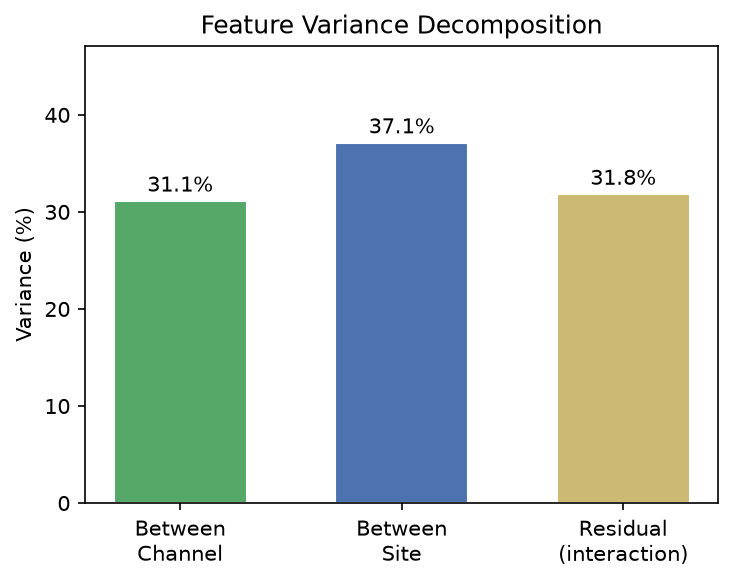
\includegraphics[width=\columnwidth]{figures/variance_decomp.png}
    \caption{Variance decomposition of the cached DINOv3 tokens on plate BR00116991: between-channel, between-site and residual components.}
    \label{fig:variance}
\end{figure}

\begin{figure}[t]
    \centering
    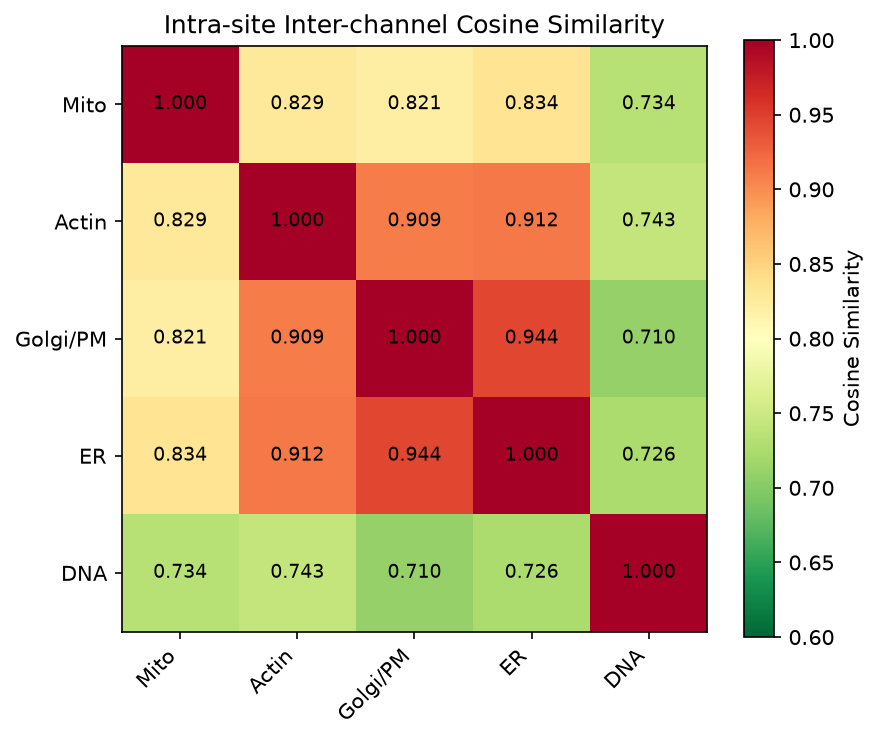
\includegraphics[width=\columnwidth]{figures/channel_similarity.png}
    \caption{Mean cosine similarity between fluorescence channels in the cached token space. The DNA channel is the most distinct.}
    \label{fig:channelsim}
\end{figure}

\begin{figure}[t]
    \centering
    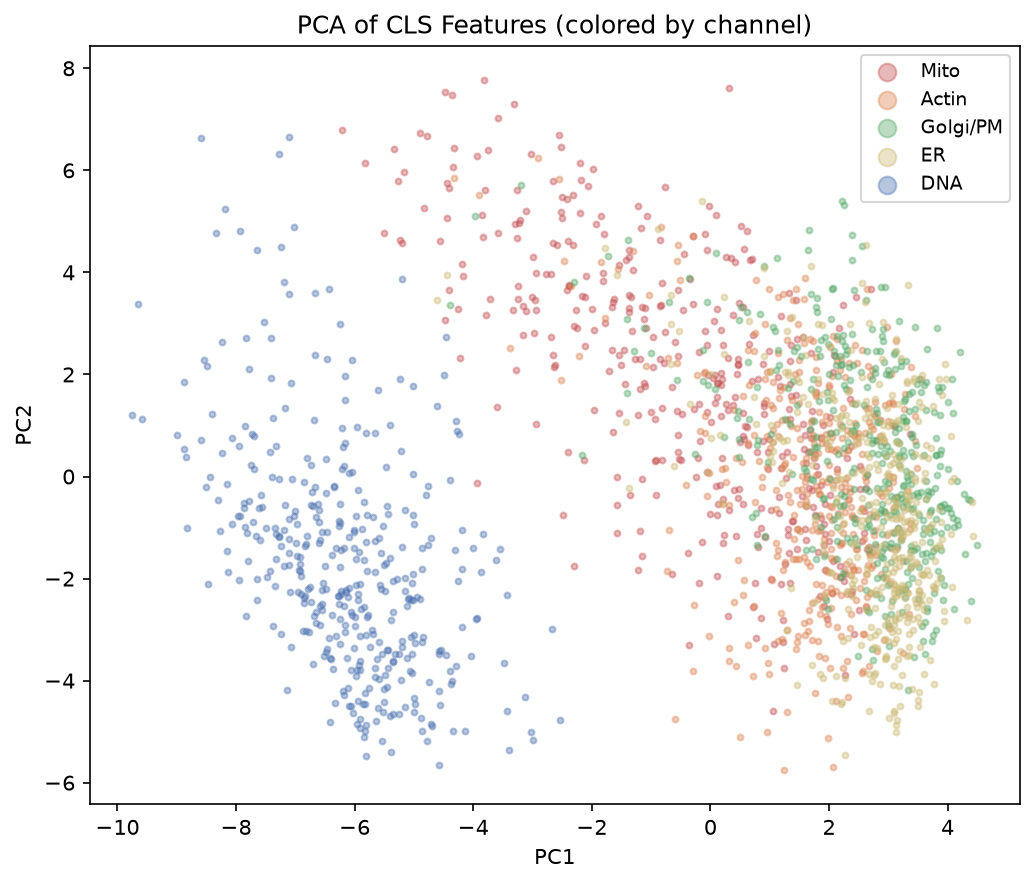
\includegraphics[width=\columnwidth]{figures/pca_channels.png}
    \caption{First two principal components of the cached 1024-d channel tokens, colored by fluorescence channel.}
    \label{fig:pca}
\end{figure}

\subsection{Cost}

For the no-offset ablation runs, \texttt{metrics.csv} records about four seconds for the training-loop phase of an epoch with 55 steps at batch size 256 on the RTX 5080. This excludes validation, data loading outside the timer and the offset-refresh pass used by offset variants, so it is not an end-to-end run-time measurement. Both backbones stay frozen; the trainable components are the CrossChannelFormer, two projection heads and one logit-scale scalar.
